% !TeX spellcheck = en_GB
\section{Question 1}

\subsection{A)}
\begin{quote}
	\textit{"Consider	Apache	Flink: \url{https://flink.apache.org}.	You	should	characterize	this	system,	describe	how	it	can	be	used	in	the	context	of	the	Lambda	architecture	and	compare	it	with	systems	you	have	used	during	your	projects."}
\end{quote}

\newpar Apache Flink[Flink] is a streaming dataflow engine. It works in a distributed setting and makes analysis of data in motion, and data at rest easier. It incorporates multiple other systems, for machine learning, graph-analysis, and more. To further characterize Flink I will use the characterization model presented in the course.

\newpar \textbf{Datamodel:} Flink works on event-based streams of data. The specific format of the events are Java and Scala embedded objects. These streams can either be infinite such as a sensor which continuously sends data, or finite such as a file. Kapfka which is a stream gathering and storing framework based on HDFS, is used by Flink to get its stream of events\cite{confluent-flink}. If events come out of order in real-time, Flink is able to sort them based on logical time instead, which can greatly simplify for example windowed computations.

\newpar \textbf{Partition Management:} To be able to scale, Flink partitions the computations on multiple nodes, which can be placed on the same server or distributed on multiple machine on a network. This approach is different from working with data in rest, where the partitioning is based on the data itself. Flink works with streams and as such, partitions the computations instead and the data/events flow between those computation nodes. Flink automatically tries to optimize the placement of the operations nodes, such that the overhead of sending the events through the network is minimized\cite{official-flink}.

\newpar \textbf{Failure handling:} Flink supports replaying of a stream to be able to recover from failures, that is if a failure occurs the stream is replayed from the last checkpoint.

The checkpoint mechanism is different from what most other big data systems use as a fall-back mechanism. The state of the nodes is periodically persisted on HDFS or in memory, such that in case of a failure replaying from that checkpoint is possible. The algorithm behind the checkpoint barriers is based on the snapshot algorithm by Chandy and Lamport\cite{data-artisan-flink}, such that the checkpoint is serially consistent across the distributed nodes, and it is not necessary to duplicate information. Once all data has flown through the barrier/checkpoint the computation is done and the computation between checkpoints either succeeds or fails atomically as a whole. The flow of the events are never held back or stopped by the checkpoint mechanism and as such, most nodes will always be in use and bottlenecks on some nodes should not hinder other nodes to d their calculations. The flow of the events happen in a directed acyclic graph structure which also means that the consistency is strong since any parallel process will always see the data in the same order\cite{data-artisan-flink}.

The checkpoint technique also separates the responsibility of calculation and failure handling, since changing the frequency of checkpoints does not alter the results of the stream.

\newpar \textbf{Batch and Stream Processing:} Flink provides two APIs, one for batch analysis and one for stream analysis. Since Flink only works on streams of data, batch processing has just been implemented as \textit{finite} stream processing. This makes Flink a framework which is based on the concept of queries at rest, instead of data at rest. An advandtagde with this approach is also that the processing code can in a lot of cases be reused for both streaming and batch views. The two API's can be used from Java or Scala, and they provide an interface much like the Java 8's Stream library\footnote{ \url{https://docs.oracle.com/javase/8/docs/api/java/util/stream/package-summary.html}}, where it is easy to do SQL-like commands, such as \texttt{where}, \texttt{groupby}, \texttt{sum} and so on. Furthermore Flink supports streaming windows over both time or counts which allows for more sophisticated analysis. As explained in the partitioning section, the different operations are distributed over a network of nodes, which each have a specific responsibility in the computation of the view.

\newpar \textbf{Throughput:} Flink prides itself with being low latency by having a powerful API to do stream processing, and by offloading some of the batch processing to the stream processing. What the streaming analysis does for low latency the ability to send information quickly forth to batch analysis, as well as the ability to scale horizontally allows for high throughput. Of course, any system which builds on top of layers of abstraction will have some latency which is not present when working on the bare metal.

On data-artisan.com\footnote{ \url{http://data-artisans.com/wp-content/uploads/2015/08/grep_throughput.png}} a graph of the throughput of different big data system is made. On figure \ref{fig:flink_bench} the graph can be seen. The strengths of Flink become very apparent, and as we can see in this case the throughput is many times higher than for example storm, which is also known for its high throughput. Flink even has a lower latency, than any of the other measured frameworks. This example is on a computation which doe snot require any reshuffling of data, and on another example the website shows a graph where the latency is noticeably higher than storm for example. Therefore the performance greatly varies based on the wanted computation.

\begin{figure}[H]
	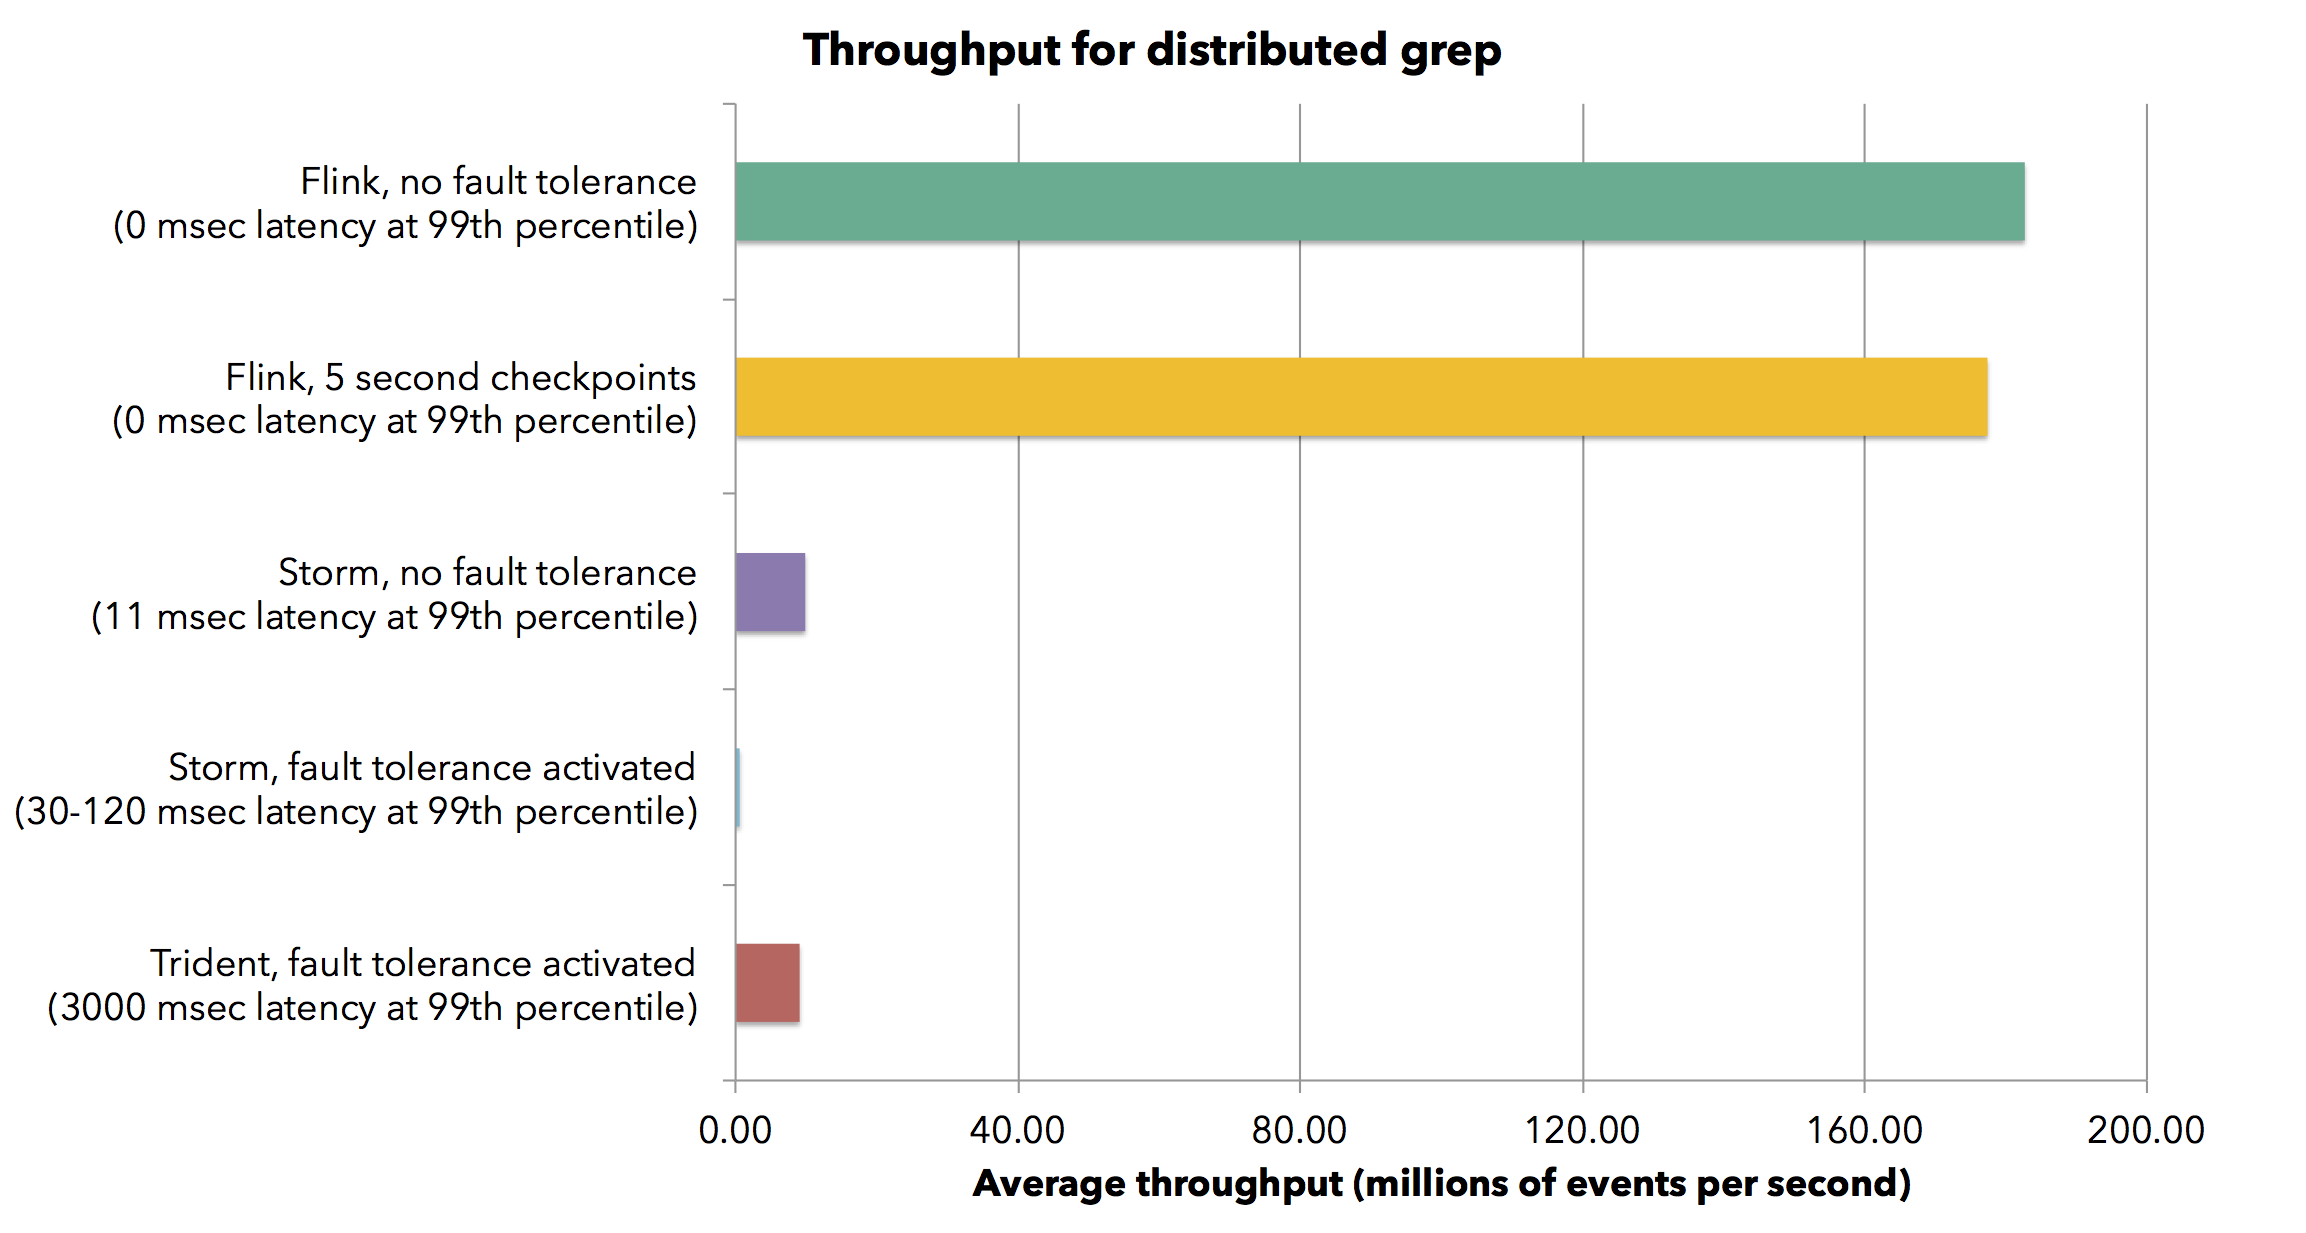
\includegraphics[width=\linewidth]{figures/flink_throughput.png}
	\caption{A graph showing the performance of different big data processing frameworks.}
	\label{fig:flink_bench}
\end{figure}

\newpar Interestingly enough Flink compares very well to the Lambda architecture. The Lambda architecture as introduced in the course, is separated into the following parts; the data sources, the master dataset, the batch layer, the serving layer, the speed layer and the queries. At the batch layer, batch views are computed, and similarly at the speed layer streaming analysis is done, and therefore it becomes quite clear that Flink naturally fits the lambda architecture by being able to be the main framework for each of these layers.

One point where the two are less alike are that Flink only works in terms of queries at rest, even in the batch layer, whereas the batch layer is in the lambda architecture described as data in rest with the processing \textit{moving} over the data.

\newpar For project 2 and 3, we could have made both batch jobs and streaming jobs, but decided to only develop batch jobs. Most of our batch jobs are made out of logic which could be expressed as -\texttt{where}, -\texttt{join} and -\texttt{groupby} statements which are available with Flink. Therefore it would be possible to have written the batch views with the Flink APIs, and have gained higher parallelism, and furthermore had the ability to with ease introduce a speed layer which could do similar calculations, but allow for lower latency from data to queries.

\subsection{B)}
\begin{quote}
		\textit{"You	are	asked	to	store	a	master	data	set	of	80	GB	given	to	you	as	an	XML	file.	Why	is	the	XML	data	format	problematic	when	working	with	Map-Reduce?	Would	a	format	transformation	from	XML	to	JSON	be	helpful?	Would	a	transformation	from	XML	to	CSV	be	helpful?	How	would	you	store	this	master	data	set?	Explain	your	answers"}
\end{quote}
The XML format is a tree structure format, and might not be easily be partitioned into smaller parts, which can be distributed among the data nodes of the storage system that Map-Reduce works on (HDFS). Furthermore XML is also a very verbose format and therefore data will take up more space which will make the transfer of data somewhat slower and require more space on the server. Even though Hadoop of course handles this quite fine, using less space is always to be preferred when the information is virtually the same. 

Transforming the data to JSON would mostly help with the amount of data, since JSON is less verbose than XML. JSON also allows for tree-structure objects and therefore partitioning can still be difficult. Since JSON objects do not specify a start and an end tag it can actually be more difficult to split up than XML. 

\newpar CSV on the other hand is a flat data structure and therefore is easily partitioned per line and split across multiple machines. Appending new data is also easy since each row is self-contained, it can be added to any data node, and therefore it is easy to do load balancing. Furthermore CSV has the advantage that it is not very verbose and it is easy to extend the input with more columns if needed.

Another possibility that we have used in Project 2 is to use a binary format. We used the serialization framework Avro\footnote{\url{https://avro.apache.org/}} for this. By choosing to use a binary format, you can represent numbers as actual numbers and not text, therefore cutting down on the needed space. Furthermore if done properly it is still possible to make the format flat and therefore making partitioning easier. This approach of course requires more work to be done, and also enforces a scheme on the data, which makes it more difficult to extend the system later on.

\newpar For project 3 we converted the data to a CSV format and stored it using Hive since it was well integrated. Hive stores the CSV data as distributed files on HDFS but uses an abstraction layer which makes the access like a regular database access. Hive allowed us to make all the views we needed and therefore it seemed like a good choice to store the data. 

It is important to notice that as soon as one transforms data, it per definition becomes derived data. Therefore, the master data set will be derived if stored in another format than it originally was, which asks the question on what to do with the primary data. I will argue that a transformation can be done from XML to CSV, which allows one to go through a similar process which converts the resulting CSV back into XML data. Even though the resulting data is not the same, it is equal to the primary data, and therefore just keeping the CSV and not the primary data is enough.

\subsection{C)}
\begin{quote}
	\textit{"Describe	pros	and	cons	of	using	the	Hadoop	ecosystem,	based	on	the	lessons	you	learnt	from	project	2	and	project	3."}
\end{quote}

The Hadoop ecosystem, has changed the industry, and how it looks at data in general. By going from a restricted view, the big data movement tries to break the boundaries but it is still very much in its youth. The relational databases go back to the 1970s and have had many years to polish its rough edges and making it easily available to developers. The big data movement is still trying to do this and most frameworks in the Hadoop data system exactly tries to sell themselves on their easy of use, but in my experience most of these systems still have a high learning curve. 

Setting up a server with a Hadoop ecosystem requires a lot of time. Systems like Horton tries to make this process easier by creating a single entry point for organizing and managing the large amount of the different Hadoop frameworks which are often required to have a complete big data system with on par functionality as a relational database system. 

\newpar Another con that we experienced when working with the Hadoop ecosystem is that integrating different frameworks is often difficult. Since standards seldom exist, frameworks are made to integrate well with other specific frameworks, but if it is desired to integrate with another system then the developers are often left to figure how to do that themselves if it is even possible.

\newpar For small systems, or embedded systems where the amount of data is know and will never surpass the amount of memory on the system (The limit of memory on most consumer hardware is around 64GB), using local computation power will be faster since it does not require any distribution of data. A lot of the frameworks also have a lot of overhead on what they do, even though they scale better. Therefore in certain systems going with a SQLite database or a system specific Relational Database would be the best solution. 

\newpar That said, the Hadoop ecosystem really shines when it comes to large amounts of data. A lot of businesses saw a huge rise in the amount of data they stored through the 2000s with the rising popularity of the internet, and now that processors were nearing their clock speed limit, being able to scale systems horizontally were very important. The Hadoop ecosystem is build around concepts of being able to abstract the distributiveness of the data away and allow developers to write code which automatically would scale to an large amount of machines in a warehouse. 

Facebook has neared the limit of the maximum amount of data that the core Hadoop ecosystem could handle. They had a data warehouse with 100 petabytes of data. The current problem with Hadoop is that the machines needs to be placed in the same warehouse to share the data over the network, without spending too much time on sending the data\cite{limit-hadoop}.

By being able to handle these large volumes, data becomes available to analysis and examination, which is one of the most important concepts of big data.

\newpar One of the pros that we experienced was how well abstracted the interfaces to most of the frameworks was. When you use Hive for example you do not have to think about how the data is distributed because the system itself will do that for you, and therefore you minimize the chances of making mistakes. Of course having extensive knowledge of the system allows you to fine tune the system even more.

\newpar The Hadoop ecosystem also focuses a lot on failure handling, such that even in the case of machine breakdowns the frameworks should be able to gracefully handle it and be able to replay, reroute, or abandon the process, and the developers are able to specify which approach should be taken as to how to restore the data of the crashed machine. 

\newpar For a lot of developers it has also been a deciding factor that the Apache foundation requires its projects to be open-source, which encourages developers to help find bugs, and ensures that the system does not require any proprietary frameworks, operating systems, or hardware.

\newpar To conclude on this it becomes obvious that if a system is going to scale, it is a good idea to use the Hadoop ecosystem since other systems might not be able to handle the same amounts of data, but if the system is of limited scale, the overhead of using the Hadoop ecosystem is quite high.
